\documentclass{beamer}
\usetheme{umbc4}
\usetheme{Boadilla}

\usepackage[absolute,overlay]{textpos} 
\newenvironment{reference}[2]{% 
  \begin{textblock*}{\textwidth}(#1,#2) 
      \footnotesize\it\bgroup\color{red!50!black}}{\egroup\end{textblock*}} 
      
% items enclosed in square brackets are optional; explanation below
\title[A short proof]{A short proof of Fermat's Last Theorem}
\subtitle[Errors]{Estimation of numerical errors}
\author[R. Rostamian]{Rouben Rostamian}
\institute[UMBC]{
  Department of Mathematics and Statistics\\
  University of Maryland, Baltimore County\\
  Baltimore, Maryland 21250\\[1ex]
  \texttt{rostamian@umbc.edu}
}
\date[November 2004]{November 26, 2004}

\begin{document}

%--- the titlepage frame -------------------------%
\begin{frame}[plain]
  \titlepage
\end{frame}

%--- the presentation begins here ----------------%
\begin{frame}{Overview}
  Overview of the material.
\end{frame}

\begin{frame}{Graphics} 
 
Here we include three images, one each of PDF, PNG, and JPG types. 
 
\begin{center} 
  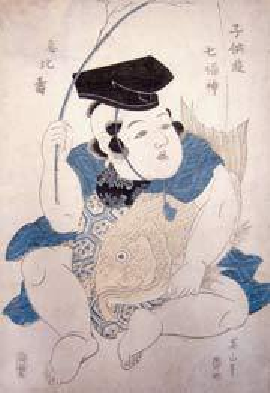
\includegraphics[width=0.3\textwidth]{image1.pdf} 
  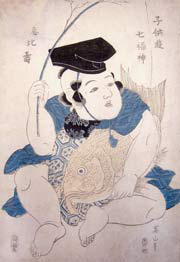
\includegraphics[width=0.3\textwidth]{image2.png} 
  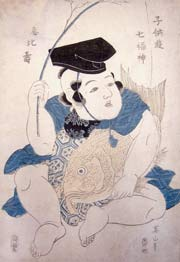
\includegraphics[width=0.3\textwidth]{image3.jpg} 
\end{center} 
 
\end{frame}


\begin{frame}[label=intro]{Outline of the talk} 
 
\begin{itemize} 
  \item Introduction 
  \pause 
  \item Statement of the main theorem 
  \pause 
  \item Technical lemmata 
  \pause 
  \item Proof of the main theorem 
  \pause 
  \item Conclusions 
\end{itemize} 
 
\end{frame} 

\begin{frame}{Some other slide}

If you click \hyperlink{intro}{here}, you will jump to the slide
labeled ``intro''.

\bigskip

Clicking \hyperlink{intro}{\beamerbutton{here}} will also
take you to the ``intro'' slide.

\end{frame}

\begin{frame}{Theorems and such}

\begin{definition}
  A triangle that has a right angle is called
  a \emph{right triangle}.
\end{definition}

\begin{theorem}
  In a right triangle, the square of the hypotenuse
  equals the sum of the squares of the two other sides.
\end{theorem}

\begin{proof}
  We leave the proof as an exercise to our astute reader.
  We also suggest that the reader generalize the proof to
  non-Euclidean geometries.
\end{proof}

\end{frame}

\begin{frame}{Title}
   \begin{reference}{4mm}{85mm}
       V. Jikov, S. Kozlov and O. Olenik, Homogenization
       of differential operators and integral
       functionals, Springer, 1994.
   \end{reference} 
  
   This is a test.
\end{frame}

\begin{frame}{Splitting a slide into columns}

The line you are reading goes all the way across the slide.
From the left margin to the right margin.  Now we are going
to split the slide into two columns.
\bigskip

\begin{columns}
  \begin{column}{0.5\textwidth}
    Here is the first column.  We put an itemized list in it.
    \begin{itemize}
      \item This is an item
      \item This is another item
      \item Yet another item
    \end{itemize}
  \end{column}

  \begin{column}{0.3\textwidth}
    Here is the second column.  We will put a picture in it.
    \centerline{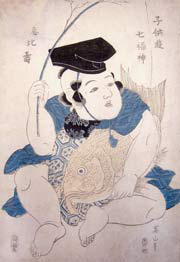
\includegraphics[width=0.7\textwidth]{image2.png}}
  \end{column}
\end{columns}
\bigskip

The line you are reading goes all the way across the slide.
From the left margin to the right margin.

\end{frame}

\end{document}